\documentclass[12pt,a4paper,fleqn]{article}
\usepackage[utf8]{inputenc}
\usepackage[russian]{babel}
\usepackage{amssymb, amsmath, multicol}
\usepackage{enumitem}
\usepackage{lipsum}
\usepackage{euler}
\oddsidemargin=-15.4mm
\textwidth=190mm
\headheight=-32.4mm
\textheight=277mm
\parindent=0pt
\parskip=8pt
\pagestyle{empty}
\usepackage{graphicx}
\title{\textbf{\LARGE{Исследовательская работа по теме:\\Исследование функции дифференциальными методами}}}
\author{Известный гражданин}
\date{November 2022}
\addt\captionsrussian{\def\refname{Список литературы}}\begin{document}
\maketitle
\newpage\newpage \textbf{\LARGE{Глава I. Функция}}

\begin{center}
$y = $$sin(x)$

\end{center}
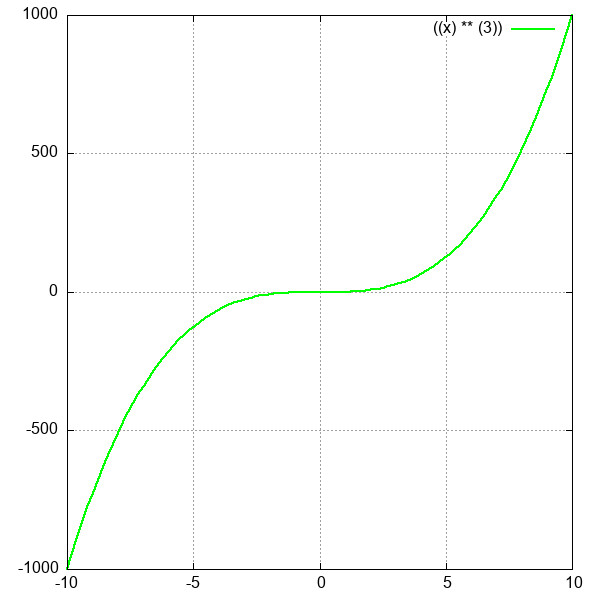
\includegraphics{GraphicDumps/plot.jpg}\newpage \textbf{\LARGE{Глава II. Визуальный анализ функции}}

Если вы понимаете данный переход, то я вам сочувствую

\begin{center}
$y = $$sin(x)$

\end{center}
\newpage \textbf{\LARGE{Глава III. Дифференцирование}}

ИИИИЕЕЕЕсли\cite{link3}

\begin{center}
 ($x)'
  = 1$\end{center}
Обоснование этого пререхода предостовляется читателю в качестве несложного упрожнения

\begin{center}
 ($sin(x))'
  = 1 \cdot cos(x)$\end{center}
DUMP

$1 \cdot cos(x)$DUMP
\newpage \textbf{\LARGE{Глава IV.Упрощение выражения}}

Для любого эпсилон больше нулю очевидно, что

\begin{center}
$1 \cdot cos(x) = cos(x)$\end{center}
\newpage \textbf{\LARGE{Глава V. Полученая производная}}

$y = $$sin(x)$

$y' = $$cos(x)$

\includegraphics{GraphicDumps/plot_1.jpg}\newpage \textbf{\LARGE{Глава VI. Разложение функции по формуле Тейлора}}

Как будет доказано в следующем семестре

\begin{center}$sin(0) = 0$\end{center}
Дифференциал - серебро, производная золото\cite{link2}

\begin{center}
 ($x)'
  = 1$\end{center}
Как будет доказано в следующем семестре

\begin{center}
 ($sin(x))'
  = 1 \cdot cos(x)$\end{center}
Дифференциал Елена всего в 100 метрах от вас...

\begin{center}
$1 \cdot cos(x) = cos(x)$\end{center}
Доказательство данного факта предоставлено лицом или организацией исполняющей функции иностанного агента

\begin{center}$cos(0) = 1$\end{center}
\\ title{не сложно заметить} 

\begin{center}
$x-0 = x$\end{center}
Как было показано ранее

\begin{center}
$x^{1} = x$\end{center}
Доказательство данного факта предоставлено лицом или организацией исполняющей функции иностанного агента

\begin{center}
 ($x)'
  = 1$\end{center}
Продвинутый читатель уже заметил, что

\begin{center}
 ($cos(x))'
  = 1 \cdot (0-sin(x))$\end{center}
Таким образом

\begin{center}
$1 \cdot (0-sin(x)) = 0-sin(x)$\end{center}
Не так страшна производная, как её находят\cite{link2}

\begin{center}$sin(0) = 0$\end{center}
Отметим, что

\begin{center}$0-0 = 0$\end{center}
Для любого эпсилон больше нулю очевидно, что

\begin{center}
$x-0 = x$\end{center}
Как будет доказано в следующем семестре

\begin{center}
 ($0)'
  = 0$\end{center}
Я придумал поистине удивительное доказательство этого факта, но поля этой книги слишком малы\ldots

\begin{center}
 ($x)'
  = 1$\end{center}
Дураку понятно, что

\begin{center}
 ($sin(x))'
  = 1 \cdot cos(x)$\end{center}
Доказательство данного факта предоставлено лицом или организацией исполняющей функции иностанного агента

\begin{center}
 ($0-sin(x))'
  = 0-1 \cdot cos(x)$\end{center}
Отметим, что

\begin{center}
$1 \cdot cos(x) = cos(x)$\end{center}
Доказательство данного факта предоставлено лицом или организацией исполняющей функции иностанного агента

\begin{center}$cos(0) = 1$\end{center}
Положим

\begin{center}$0-1 = -1$\end{center}
Функция производной не стоит\cite{link2}

\begin{center}
$x-0 = x$\end{center}
\textbf{\LARGE{Получим разложение по формуле Тейлора:}}
\begin{center}
$y = $$0+((\frac{1}{1}) \cdot x+((\frac{0}{2}) \cdot x^{2}+(\frac{-1}{6}) \cdot x^{3}))$$ + o((x - 0.000000)^{3})$
\end{center}
\newpage\begin{thebibliography}{}
\bibitem{link1}  "A Synopsis of Elementary Results in Pure and Applied Mathematics"
\bibitem{link2}  "Сборник пословиц и поговорок под редацией кафедры высшей математики"
\bibitem{link3}  "Полное собрание лучших высказываний преподавателей МФТИ"
\bibitem{link4}  "Словарь фраз, не несущих смысловой нагрузки. 17 издание"
\end{thebibliography}\end{document}